\chapter{Explicitly Correlated Methods}
\label{chap:explicit}

With the advent of modern computers combined with a vast array of sophisticated algorithms from which to choose, \emph{ab initio} quantum chemistry has become a tremendously powerful tool, going beyond the study of small atoms, to molecules and solids, and are among the most effective and systematically improvable techniques to date. Nevertheless, convergence to the \gls{CBS} limit is notoriously slow.

In particular, consider the popular basis set family developed by Dunning and coworkers, \gls{cc-pV$X$Z}.\cite{dunningGaussian1989,woonGaussian1993,woonGaussian1994,petersonBenchmark1994,wilsonGaussian1996}
The size of these basis sets scale as $M\in\mathcal{O}(X^3)$, and since for standard post-Hartree-Fock discussed in chapter \ref{sec:post-hf} we require four-index integrals, our computation time will scale at best as $t\in\mathcal{O}(X^{12})$.\cite{klopperR122007}
% TODO ? should I include this equation?
% $$\sum_{n=1}^X \sum_{l=0}^{n-1} (2l+1) = \frac{X(X+1)(2X+1)}{6}$$
% explains the scaling

Meanwhile, the \gls{CBS} correlation error scales as $\epsilon\in\mathcal{O}(X^{-3})$ \cite{helgakerBasisset1997,halkierBasisset1998} or $\epsilon\in\mathcal{O}(M^{-1})$,\cite{klopperInitio1995} resulting in time $t\in\mathcal{O}(M^{-\frac 14})$. Thus, the methods discussed so far come with the painful cost of requiring very large basis sets to approach high-accuracy results.

Explicitly correlated methods are a class of electronic structure methods specifically designed to address this unfavourable scaling by explicitly including the interelectronic distance $r_{12}$, and is the subject of this chapter. As the R12/F12 family of methods is the most mature of the explicitly correlated electronic structure methods, many reviews focusing on this topic already exist. This chapter in particular is in large part based on references \parencite{klopperR122007,gruneisPerspective2017,hattigExplicitly2011,shiozakiMultireference2013}.

% \textcite{klopperR122007,gruneisPerspective2017,hattigExplicitly2012,shiozakiMultireference2013}.

% three reviews: references \citenum{klopperR122007}, \citenum{gruneisPerspective2017} and \citenum{hattigExplicitly2012}.


\section{The Cusp Conditions}
\label{sec:cusp}

Consider two charged point particles in a system described by the Hamiltonian of equation \eqref{eq:elec_hamiltonian_2q}. By the Schr\"odinger equation, the local energy
\begin{equation}
    E_L\mathdef \frac{H\Psi}{\Psi}
\end{equation}
must be constant in the exact solution. However, when these two particles coalesce, i.e. $r_{12}\to 0$, the Coulomb potential, $r^{-1}$, diverges. Thus, for the local energy to be constant, we must have that near coalescence points, the kinetic energy exactly cancels the Coulomb energy. A more formal treatment of this argument leads to the (antiparallel) electron-electron Kato cusp condition,\cite{katoEigenfunctionsManyparticleSystems1957a}
\begin{equation}
    \label{eq:cusp}
    \left.\widetilde{\frac{\partial \Psi}{\partial r_{12}}}\right|_{r_{12}\to 0}
    = \frac 12 \Psi(r_{12}=0)
\end{equation}
where the tilde represents spherical averaging.

This cusp condition was also later generalised.\cite{packCuspConditionsMolecular1966,kurokawaChapterTwoGeneral2016}
Early literature on the subject suggested that the success of explicitly correlated methods were due to the superior description of short-range correlation effects, and in particular in their much more faithful capturing of the cusp conditions like equation \ref{sec:cusp}.\cite{roothaanAnalytical1960,watsonApproximate1960,weissConfiguration1961,schwartzGround1962}
However, further study found that the correlation error from a bad description of the wave function around a small sphere centred on the cusp is actually negligible.\cite{coulsonElectron1961,gilbertInterpretation1963,prendergastImpact2001,klopperR122007} Instead, the success of explicitly correlated methods is actually due to the superior description of the overall shape and size of the Coulomb hole, which has a radius on the order of the atomic radius.

To understand why gaussian-type basis sets fail so spectacularly at capturing the cusp behaviour, it is instructive to consider a simpler example, like that of approximating $|x|$ by its Fourier decomposition. Such an illustration is found in figure \ref{fig:cusp}. It is also worth noting that \glspl{STO} do not suffer as badly from this limitation,\cite{kongExplicitly2011} but as discussed in chapter \ref{sec:orbitals}, they are unsuccessful due to their lack of practicality.\footnote{Note that \glspl{STO} do not suffer from the electron-nuclear cusp, which is in any case not the focus of many explicitly correlated methods, such as F12, as discussed later in this chapter. Even with \glspl{STO}, we have electron-electron cusps.}

\begin{figure}[htbp]
    \centering
    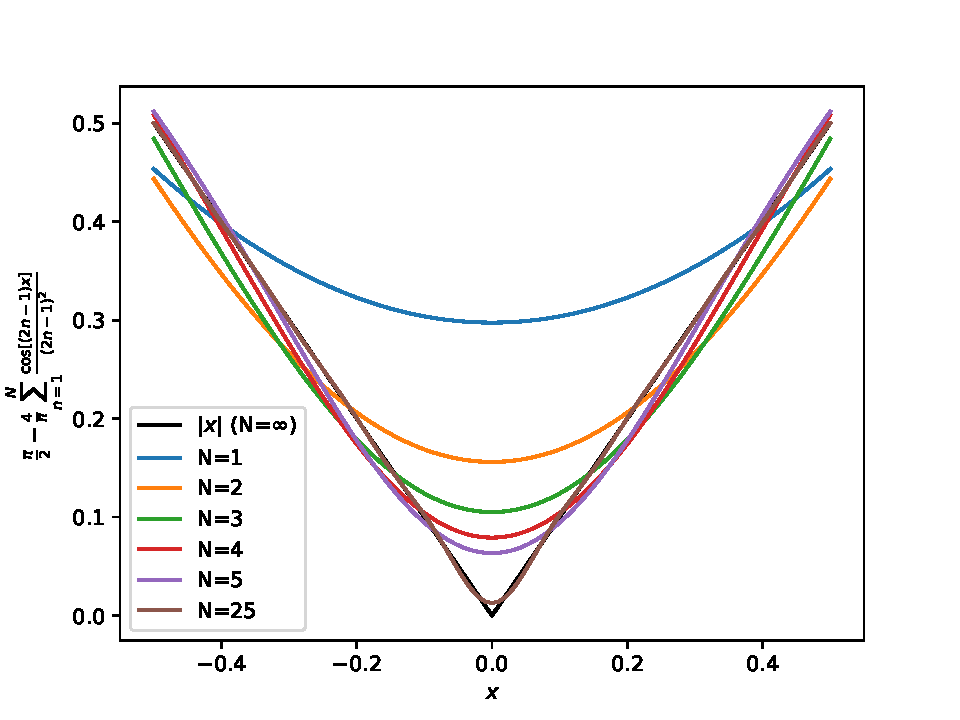
\includegraphics{figures/explicit/cusp.pdf}
    \caption{A toy example of the Coulomb cusp. Here, the Fourier expansion $x\approx\frac{\pi}{2} - \frac {4}{\pi} \sum_{n=1}^N\frac{\cos[(2n-1)x]}{(2n-1)^2}$ is plotted for a few values of $N$, including the exact solution. As can be seen, even for many terms, the Fourier expansion is a poor descripter in the cusp region. Indeed, the only way to describe it exactly is with an infinite number of terms.}
    \label{fig:cusp}
\end{figure}

\section{Hylleraas Methods}

Almost 30 years prior to Kato's landmark paper describing cusps in the analytical form for the wave function, there was already work being done to understand the significance of including $r_{12}$ terms in the wave function. Instead of being motivated by rigorous mathematics like Kato's, Slater was motivated by studies in the He atom. In particular, he tried to construct a wave function which faithfully represents both the core region as well as the Rydberg limit (i.e. a highly excited atom where the electron is very far from the nucleus).\cite{kongExplicitly2011,grynbergIntroduction2010,slaterCentral1928,slaterNormal1928} This led him to suggest multiplying the wave function by a factor
\begin{equation}
    \e^{-2(r_1+r_2)+r_{12}/2},
\end{equation}
which can easily be shown to satisfy the cusp equation \eqref{eq:cusp}.

However, the first successful explicitly correlated electronic structure calculation is typically attributed to Hylleraas,\cite{hattigExplicitly2011} where he aimed to improve convergence of orbital expansions for helium.\cite{hylleraasUeber1928,hylleraasNeue1929} In this method, the coordinates $s\mathdef r_1+r_2$, $t\mathdef r_1 - r_2$ and $u\mathdef r_{12}$ are used to construct the wave function
\begin{equation}
    \Psi_N(s,t,u) = \e^{-\alpha s}\sum_{k}^N c_ks^{l_k}t^{2m_k}u^{n_k}.
\end{equation}

In particular, using only three terms ($N=3$), and variationally optimising for the parameters $c_1,c_2,c_3$, Hylleraas was able to reach within 1.3 millihartree from the exact result.

Since then, there was rapid development on this approach and combining it with \gls{CI} (which came to be known as the CI-Hyl methods).
\cite{largo-cabrerizoHylleraasCI1987,jamesGround1933,kolosAccurate1964,perkinsAtomic1968,perkinsAtomic1969,simsCombined1971,simsOneCenter1971,claryHylleraastype1977,claryCIHylleraas1976} In CI-Hyl methods, the wave function is expanded as in \gls{CI},
\begin{equation}
    \Psi = \sum_k c_k \Phi_k
\end{equation}
where
\begin{equation}
    \Phi_k = \mathcal{A} r^{\nu_k}_{ij}\prod_i\chi_{k_i}(\bm x_i)
\end{equation}
where ${\chi_k}$ is a spin-orbital basis and $\mathcal{A}$ is the antisymmetriser operator.

However, CI-Hyl methods were to eventually fall out of favour. This is because the expansions involve exceedingly difficult integrals involving many electrons and over products of correlation factors. This significantly restricts the tractibility and scalability of the method, and it has since largely gone unused.

\section{Explicitly Correlated Gaussians}

Boys\cite{boysIntegral1960} and Singer\cite{singerUse1960} independently introduced gaussian basis functions with explicit correlation for calculations on molecules.\cite{mitroyTheory2013} These methods are referred to as \glspl{ECG}, or in the case of functions of two electrons, \glspl{GTG}. A spherical \gls{GTG} may be written (with nuclar coordinates $\bm R_1$ and $\bm R_2$) as
\begin{equation}
    g(\bm r_1, \bm r_2) = \exp(-\zeta_1|\bm r_1 - \bm R_1|^2 - \zeta_2|\bm r_2 - \bm R_2|^2 - \gamma|\bm r_1 - \bm r_2|^2).
\end{equation}
This can be interpreted as two $s$-type orbitals and an interelectronic correlation factor $\e^{-\gamma r_{12}^2}$.
While they do not have the correct cusp behaviour, a linear combination of \glspl{GTG} approximately capture the electron-electron cusp. This is similar to how gaussian basis functions do not individually capture the electron-nuclear cusp, but a linear combination of them approximately does.

One major strength of this approach is that all integrals have closed-form algebraic expressions,\cite{lesterGaussian1964} and avoids nonlinear optimisation.\cite{bukowskiNew1994,perssonAccurate1996} \Gls{ECG} methods have been extended to post-Hartre-Fock methods, such as MP2\cite{panGaussian1970,panElectron1972}, and methods to avoid its many difficult integrals have also been developed.\cite{szalewiczNew1982,szalewiczAtomic1983,wenzelAtomic1986,szalewiczAtomic1984,tewWeak2007}

While not as popular as F12 methods (see section \ref{sec:f12}), \glspl{ECG} have been used for highly accurate variational calculations,\cite{korobovCoulomb2000} as well as for applications outside of standard electronic structure theory, such as bosons,\cite{vargaPrecise1995} positronium (a bound state of an electron and a positron),\cite{bubinGroundstate2011} and non-Born-Oppenheimer systems.\cite{stankeNonBornOppenheimer2009}

\section{F12 Methods}
\label{sec:f12}

The most influential class of explicitly correlated methods to date are the F12 methods. The core principle of these methods is to augment the wave function from a conventional (typically \gls{SD}) basis with an explicitly-correlated correction, called the F12 (or R12) correction. The original formulation\supercite{kutzelnigg12Dependent1985} parametrised a two-electron system (such as helium) wave function as
\begin{equation}
    \label{eq:first-r12}
    \ket\Psi = (1+tQ_{12}F_{12}(r_{12}))\ket{\Psi_0}+\sum_{p}t_{p}\ket{\Psi_{p}}
\end{equation}
where $\Psi_0$ is a reference wave function (such as \gls{HF}), $\ket{\Psi_{p}}$ are excited-state \glspl{SD}, $t,t_{p}$ are parameters (``amplitudes'') to be optimised, and
\begin{equation}
    Q_{12} \mathdef \sum_{\alpha\beta}\ket{\alpha\beta}\bra{\alpha\beta}
\end{equation}
is referred to as a ``strong orthogonality projector'', which ensures the $F_{12}(r_{12})$ term is orthogonal to the reference and singly-excited determinants.
Here $\alpha,\beta$ refer to virtual orbitals in the formally complete basis. The fact that, due to $Q_{12}$, the $F_{12}(r_{12})$ term commutes with the standard excitation operators aids in including this explicit correlation into conventional electron correlation methods. This geminal term is added a correction to the standard wave function.
% NOTE TO self: when defending, might want to review Joachim Werner's F12 review to properly understand this form of writing Q12

In the original formulation, $F_{12}(r_{12})=r_{12}$ (hence the name ``R12'' or ``F12'' for the more general methodology). However, another popular choice is a Slater-type geminal\supercite{ten-noInitiation2004} fitted to a linear combination of gaussians,\supercite{wernerGeneral2007}
\begin{equation}
    \label{eq:f12-exponential}
    F_{12}(r_{12})=-\gamma^{-1}\e^{-\gamma r_{12}} = -\gamma^{-1}+r_{12}-\frac 12\gamma r_{12}^2+\cdots \approx \sum_i c_i\e^{-\alpha_ir_{12}^2}.
\end{equation}
The choice of the length scale $\gamma$ can either be optimised or (more typically) kept fix, although formally it is orbital dependent and a poor choice may result in a loss of accuracy.\supercite{tewRelaxing2018} Other choices for the correlation factor also exist.\supercite{johnsonExplicit2017}

\subsection{MP2-F12}

Following the discussion in reference \citenum{shiozakiMultireference2013}, and adopting their notation, we consider the MP2-F12 method as an illustrative example.

An alternative derivation of the \gls{MP2} equations from section \ref{sec:perturbation-theory} is to minimise the Hylleraas functional\supercite{hylleraasUeber1930,betheQuantum1957}
\begin{equation}
    \label{eq:hyllerass-functional}
    E^{(2)} = \min_\Psi\bra{\Psi^{(1)}}(H_0-E^{(0)})\ket{\Psi^{(1)}}+2\bra{\Psi^{(1)}}H\ket{\Psi^{(0)}}
\end{equation}
where $H_0$ is the unperturbed Hamiltonians, and the $(i)$ superscript denotes the order of the correction, as introduced in section \ref{sec:perturbation-theory}.

The earliest generalisation of equation \ref{eq:first-r12} was an ansatz for MP2,\supercite{klopperMollerplesset1987,kutzelniggWave1991,klopperOrbitalinvariant1991,tewOpenshell2010,bokhanImplementation2008}
\begin{equation}
    \label{eq:mp2-f12-firstorder}
    \ket{\Psi^{(1)}} = \frac 12\sum_{ij}\left( \sum_{ab}t_{ij}^{ab}\ket{\Psi_{ij}^{ab}} + \sum_{kl}t_{ij}^{kl}\sum_{\alpha\beta}\bra{\alpha\beta}Q_{12}F_{12}(r_{12})\ket{kl}\ket{\Psi_{ij}^{\alpha\beta}} \right),
\end{equation}
\begin{equation}
    \label{eq:mp2-f12-projector}
    Q_{12} = (1-o_1)(1-o_2) - v_1v_2
\end{equation}
where we define the one-electron projection operators
\begin{equation}
    o_m = \sum_i\ket{\phi_i(\bm r_m)}\bra{\phi_i(\bm r_m)}
\end{equation}
and
\begin{equation}
    v_m = \sum_a\ket{\phi_a(\bm r_m)}\bra{\phi_a(\bm r_m)}
\end{equation}
such that $o_m$ and $v_m$ project onto the occupied and virtual orbitals, respectively, with
\begin{equation}
    \bra{\phi_i(\bm r_m)}\Omega\ket{jk} = \int\d^3r_m\ \phi_i^*(\bm r_m)\Omega\phi_j(\bm r_1)\phi_k(\bm r_2)
\end{equation}
for operator $\Omega$. The first term in brackets in equation \ref{eq:mp2-f12-firstorder} are from the conventional MP2 wave function correction, and the extra term is a contraction of a formally-infinite set of double excitations, representing the F12 correction (again, orthogonal to the conventional wave function thanks to $Q_{12}$).

It was also shown that solving for the amplitudes $t_{ij}^{kl}$ can be avoided,\supercite{ten-noNew2007,tewComparison2006,wernerGeneral2007,klopperExplicitly2002,petersonBenchmark1994} and can instead be derived from the cusp conditions to give
\begin{equation}
    t_{ij}^{kl} = \frac 38\delta_{ik}\delta_{jl}+\frac 18\delta_{il}\delta_{jk}.
\end{equation}
This also tends to be more accurate, as it avoids the geminal basis set superposition error.\supercite{tewComparison2006,adlerSimple2007}

\subsection{Many-Electron Integrals}

The Hylleraas functional, equation \ref{eq:hyllerass-functional}, will contain terms such as
\begin{equation}
    \sum_{\alpha\beta}\bra{\Phi_0}H\ket{\Psi_{ij}^{\alpha\beta}} \bra{\alpha\beta}Q_{12}F_{12}(r_{12})\ket{kl} = 2\bra{ij}r_{12}^{-1}Q_{12}F_{12}(r_{12})\ket{kl} - \bra{jl}r_{12}^{-1}Q_{12}F_{12}(r_{12})\ket{kl}.
\end{equation}
Plugging in the form for $Q_{12}$ from equation \ref{eq:mp2-f12-projector}, we get integrals of the form
\begin{equation}
    \bra{ij}r_{12}^{-1}o_1F_{12}(r_{12})\ket{kl}.
\end{equation}
For $F_{12}(r_{12})=r_{12}$, this is equal to
\begin{equation}
    \sum_o\bra{ijo}r_{12}^{-1}r_{23}\ket{olk},
\end{equation}
which is a three-electron integral. Here, $o$ is an occupied orbital. Clearly, with more operators multiplied together in the kernel of these integrals, we might expect even higher-order integrals. This may seem distrastrous, as this would be a massive bottleneck.

However, it was found that by insertion of the \gls{RI},\supercite{kutzelniggR12DependentTermsWave1985,klopperMollerplesset1987,kutzelniggWave1991} these integrals can be reduced to a linear combination of two-electron integrals. In particular, the strong projection operator becomes
\begin{equation}
\begin{split}
    Q_{12} =& 1 - \sum_o\sum_\alpha (\ket{o\alpha}\bra{o\alpha} + \ket{\alpha o}\bra{\alpha o})
            + \sum_{o,o'}\ket{oo'}\bra{oo'} - \sum_{a,b}\ket{ab}\bra{ab},
\end{split}
\end{equation}
and the discussed three-body integral becomes
\begin{equation}
\begin{split}
    \sum_o\bra{ijo}r_{12}^{-1}r_{23}\ket{olk} =& \delta_{ik}\delta_{kl} \\
    &- \sum_{o}\sum_\alpha(\bra{ij}r_{12}^{-1}\ket{o\alpha}\bra{o\alpha}r_{12}\ket{kl} + \bra{ij}r_{12}^{-1}\ket{\alpha o}\bra{\alpha o}r_{12}\ket{kl}) \\
    &+ \sum_{o,o'}\bra{ij}r_{12}^{-1}\ket{oo'}\bra{oo'}r_{12}\ket{kl}
    - \sum_{a,b}\bra{ij}r_{12}^{-1}\ket{ab}\bra{ab}r_{12}\ket{kl}.
\end{split}
\end{equation}
In the \gls{RI} approximation, the summation over the additional orbitals $\alpha$ is in principle infinite. In practice, of course, these must be finite. Initially, the basis in the \gls{RI} expansion was set equal to the orbital basis (dubbed the ``standard approximation'').\supercite{kutzelniggR12DependentTermsWave1985,klopperOrbitalinvariant1991,klopperMollerplesset1987,klopperMP2R12,kutzelniggWave1991,termathWave1991,windSecondorder2002,valeevImproving2004,klopperWave1991} However, normally larger bases are used, such as in the \gls{CABS} approach, where the \gls{RI} basis is equal to the orbital basis, plus some ``auxiliary'' basis functions that are orthogonal to the orbital basis.\supercite{klopperExplicitly2002,valeevImproving2004} Many more important advances were since made, such as more efficient RI methods and ways of generating intermediate values have also been developed.\supercite{manbyDensity2003,wernerGeneral2007,ten-noDensity2003,kedzuchAlternative2005,shiozakiExplicitly2008,kohnImplementation2008,shiozakiHigherorder2009,wernerExplicitly2006,manbyExplicitly2006,wernerEliminating2008,petersonSystematically2008,yousafOptimized2008,yousafOptimized2009,ten-noInitiation2004,ten-noExplicitly2004,klopperExplicitly2002,ten-noNew2007,shiozakiEvaluation2009,mayExplicitly2004,adlerLocal2009,klopperHybrid2004}

Moreover, it has been found that the original $F_{12}(r_{12})=r_{12}$ form requires larger auxiliary basis functions, since its long-range behaviour is unphysical.\supercite{ten-noInitiation2004,ten-noNew2007} Instead, functions such as that in equation \ref{eq:f12-exponential} is used.

\subsection{Higher-Order F12 Theories}

F12 theory has been extended to many other theories besides MP2, such as \gls{CC}, \gls{CASSCF}, \gls{MRCI}, \gls{CASPT2}, \gls{DMRG}, and \gls{FCIQMC}.
\supercite{shiozakiMultireference2013,nogaCCR121992,nogaCoupled1994,gdanitzFormulation1993,gdanitzAccurately1998,flieglCoupledcluster2006,neissExtensions2006,kohnModified2009,bokhanCommunications2010,hofenerExtended2019,kedzuchMultireference2011,manbyExplicitly2006,neeseEfficient2009,wernerExplicitly2017,varganovVariational2010,ten-noSimple2007,shiozakiCommunication2010,sharmaSpectroscopic2014}
The key change compared to conventional methods such as those in chapter \ref{chap:intro} is in the excitation operators, particularly the double excitations $E_{ij}^{ab}$. In particular, for a multireference method with reference determinants $\ket{\Phi_I}$, the wave function may be parametrised as
\begin{equation}
    \ket\Psi = \ket{\Psi_\text{conv}} + \frac 12\sum_{I}\sum_{ijkl}t^{ij}_{klI}\sum_{\alpha\beta}\bra{\alpha\beta}Q_{12}^IF_{12}(r_{12})\ket{kl}E_{ij}^{\alpha\beta}\ket{\Phi_I},
\end{equation}
where $\ket{\Psi_\text{conv}}$ is the conventional wave function. In this way, we extend the excitations to include geminal terms in the (formally complete) auxiliary basis.

These F12 methodologies have been particularly successful for large systems, proving only marginally more expensive than the conventional methods in some cases.\supercite{adlerSimple2007,kniziaSimplified2009}

Since F12 methods work directly on the wave function, it is also natural to extend to excited states, particularly for multireference methods.
\supercite{floresAccurately2005,ten-noSimple2007,shiozakiCommunication2010,shiozakiExplicitly2011,flieglCoupledcluster2006}
However, since the geminal terms include only occupied orbitals, there is an inherent bias to the ground state.\supercite{flieglCoupledcluster2006,neissExtensions2006} Several means of ameliorating this have been proposed, such as combining F12 with response theory,\supercite{neissExtensions2006} or by including extending the geminal basis to include virtual orbitals.\supercite{kohnModified2009}

\section{The Transcorrelated Method}
\label{sec:tc}
% Based on Haettig review, Cohen paper, Tsuneyuki paper, a tiny bit Lee paper, tiny bit from Thomasle

One of the main focuses of this dissertation is \gls{TC}. Hirschfelder was the first to propose a similarity-transformed Hamiltonian method in the 1960s,\cite{hirschfelderRemoval1963} which was further developed by Jankowski,\supercite{Jankowski1967,Jankowski1970} and later by Boys and Handy.\supercite{boysCalculation1969,boysCondition1969,boysDetermination1969,boysFirst1969}

The core concept is to similarity-transform the Hamiltonian using some invertible operator $P$, such that
\begin{equation}
    \htc = P^{-1}\hat HP.
\end{equation}
For any eigenvalue and eigenfunction pair $(E_i,\Psi)$ of $\hat H$, the transformed Hamiltonian $\htc$ has eigenfunction $\Phi\mathdef P\Psi$ with the same eigenvalue $E_i$. This is called isospectrality, and it allows us to solve $\htc$ to get the spectrum of $\hat H$.

However, note that there is no requirement that $\htc$ is Hermitian, and in fact it typically is not. Recall from section \ref{sec:variational_principle} that the variational principle relies on the Hermiticity of the operator. It is therefore nontrivial to make \gls{TC} variational, and not all conventional methods can be used to treat $\htc$ (although, as discussed in section \ref{sec:fciqmc}, projector methods such as FCIQMC and CC may be used).

\subsection{The Method of Boys and Handy}

One of the earliest practical approaches, on which most modern variations build, is that of Boys and Handy.\supercite{boysCalculation1969,boysCondition1969,boysDetermination1969,boysFirst1969} In this methodology, we start with a Jastrow ansatz\cite{jastrowManyBody1955}
\begin{equation}
    \label{eq:jastrow-ansatz}
    \Psi = \e^J\Phi.
\end{equation}
In this way, TC shares similarities with \gls{VMC}, to be discussed in section \ref{sec:vmc}. Inserting \ref{eq:jastrow-ansatz} into the Schrödinger equation, we get
\begin{equation}
    \hat H \e^J\Phi = E\e^J\Phi \implies \underbrace{\e^{-J}\hat H\e^J}_{\htc}\Phi = E\Phi,
\end{equation}
i.e. similarity-transforming $\hat H$ with the operator $P\equiv\e^J$.

In the original formulation, $\Phi$ was chosen to be a single \gls{SD} (\gls{HF}), and $J$ was chosen such that
\begin{equation}
    \label{eq:jastrow-two-elec}
    J = \sum_{i<j}u(\bm r_i, \bm r_j)
\end{equation}
where $u(\bm r_i, \bm r_j) = u(\bm r_j, \bm r_i)$ is a symmetric two-electron correlation function.

The \gls{BCH} expansion of $\htc$ truncates exactly to second order, i.e.
\begin{equation}
    \htc \mathdef \e^{-J}\hat H\e^J= \hat H + [\hat H, J] + \frac 12[[\hat H,J],J].
\end{equation}
This may be rewritten
\begin{equation}
    \htc = \hat H - \sum_{i<j}\hat K(\bm r_i, \bm r_j) - \sum_{i<j<k}\hat L(\bm r_i, \bm r_j, \bm r_k),
\end{equation}
where, using the shorthand $u_{ij} \mathdef u(\bm r_i, \bm r_j)$,
\begin{equation}
\begin{split}
    \hat{K}(\bm{r}_i, \bm{r}_j) = \frac{1}{2} \Bigg(
        \nabla_i^2 u_{ij} + \nabla_j^2 u_{ij} +
        \big(\nabla_i u_{ij}\big)^2
        + \big(\nabla_j u_{ij}\big)^2\Bigg)
        + \big(\nabla_i u_{ij} \cdot \nabla_i\big)
        + \big(\nabla_j u_{ij} \cdot \nabla_j\big)
        ,
\end{split}
\end{equation}
and
\begin{equation}
\begin{split}
\hat{L}(\bm{r}_i, \bm{r}_j, \bm{r}_k) =
\nabla_i u_{ij} \cdot \nabla_i u_{ik} +
\nabla_j u_{ji} \cdot \nabla_j u_{jk} +
\nabla_k u_{ki} \cdot \nabla_k u_{kj}.
\end{split}
\end{equation}

In second quantisation, the TC Hamiltonian can then be written
\begin{equation}
    \htc = \sum_{pq} h_q^p a_p^\dagger a_q
    + \frac{1}{2} \sum_{pqrs} \big(V_{rs}^{pq} - K_{rs}^{pq}\big)
    a_p^\dagger a_q^\dagger a_s a_r
    - \frac{1}{6} \sum_{pqrstu} L_{stu}^{pqr}
    a_p^\dagger a_q^\dagger a_r^\dagger a_u a_t a_s,
\end{equation}
where
\begin{equation}
\begin{split}
    h_q^p &= \bra{p}h\ket{q}, \\
    V_{rs}^{pq} &= \bra{p q } r_{12}^{-1} \ket{ r s}, \\
    K_{rs}^{pq} &= \bra{p q } \hat{K} \ket{ r s}, \\
    L_{stu}^{pqr} &= \bra{p q r } \hat{L} \ket{s t u}.
\end{split}
\end{equation}
Particularly noteworthy are the three-electron integrals from $\hat L$ and the non-Hermitian terms from $\hat K$.

Boys and Handy's original choice for the form of $u$ was
\begin{equation}
    \label{eq:boys-handy-jastrow}
    u(\bm r_i, \bm r_j) = \sum_{l,m,n}^{l+m+n\leq S} c_{lmn}\bar r_{ij}^l(\bar r_{Ii}^m\bar r_{Jj}^n + \bar r_{Ij}^m\bar r_{Ji}^n)
\end{equation}
where $S$ is some integer ($S=6$ in reference \citenum{boysCalculation1969})\supercite{cohenSimilarity2019} and
\begin{equation}
    \bar r = \frac{r}{1+r}.
\end{equation}
In this form, electron-electron (e-e), electron-nucleus (e-n), electron-electron-nucleus (e-e-n) and electron-electron-nucleus-nucleus (e-e-n-n) terms appear when $m=n=0$ and $l>0$, $m,n>0$ and $l=0$, one of $m,n>0$ and $l>0$, or $m,n,l>0$ respectively.

In the original formulation,\supercite{boysCalculation1969} the following equations are approximately solved via quadrature for the orbital coefficients $a_i$ and the coefficients $c_{lmn}$ in $u$.
\begin{equation}
    \bra\Phi(\htc - E)\ket\Phi = 0
\end{equation}
\begin{equation}
    \bra{\partial\Phi/\partial a_i}(\htc - E)\ket\Phi = 0
\end{equation}
\begin{equation}
    \label{eq:almost-hermitian}
    \bra\Phi(\htc - \htc^\dag)\ket\Phi = 0,
\end{equation}
and the energy is calculated via projection,
\begin{equation}
    \bra\Phi\htc\ket\Phi.
\end{equation}
Equation \ref{eq:almost-hermitian} in particular is to make the TC Hamiltonian as close to Hermitian as possible for orbital optimisation.

This formulation was further refined by Handy.\supercite{handyEnergies1969} We notice that since $\htc$ is non-Hermitian, we cannot directly minimise the energy. Instead, he minimised the transcorrelated variance,
\begin{equation}
    \sigma^2 = \langle [(\htc - E)\Phi]^2\rangle.
\end{equation}
Furthermore, equation \ref{eq:boys-handy-jastrow} is not the only possible choice for the Jastrow factor, and in particular Handy chose a form with simpler analytical integrals.


\subsection{Modern Resurgence}

For several decades TC received little attention, though some more developments were made, such as calculations using a fixed Jastrow factor,\supercite{nooijenElimination1998} more efficient integration,\supercite{ten-noFeasible2000,ten-noThreeelectron2000} multi-reference $\Phi$,\supercite{zweistraSimilarityTransformed2003} among others.\supercite{Luo2010,luoVariational2010,luoComplete2011} More recently, there has been a renewal of interest in TC,
\supercite{ammarCompactification2024,ammarExtension2022,ammarTranscorrelated2023,baiardiExplicitly2022,baiardiTranscorrelated2020,christlmaierXTC2023,cohenSimilarity2019,Dobrautz2019,dobrautzPerformance2022,dobrautzReal2024,ginerNew2021,Guther2021,hinoApplication2002,imamuraNew2003,jeszenszkiAccelerating2018,jeszenszkiEliminating2020,katsOrbital2024,kumarQuantum2022,leeStudies2023,liaoDensity2023,liaoEfficient2021,Luo2010,luoCombining2018,luoComplete2011,luoTranscorrelated2012,luoVariational2010,magnussonEfficient2024,mottaQuantum2020,ochiEfficient2012,ochiIterative2016,ochiOptical2014,sakumaElectronic2006,schraivogelTranscorrelated2021,schraivogelTranscorrelated2023,sokolovOrders2023,szenesStriking2024,ten-noNew2002,ten-noNonunitary2023,tsuneyukiTranscorrelated2008,umezawaExcited2004,umezawaGroundstate2004,umezawaPractical2005,umezawaTranscorrelated2003}
notably the demonstrations that the TC Hamiltonian may be treated by various electronic structure methods, to be discussed more in section \ref{sec:tc-fciqmc}.\supercite{luoCombining2018,cohenSimilarity2019,liaoDensity2023,baiardiExplicitly2022,ammarExtension2022,ammarTranscorrelated2023,ammarCompactification2024,schraivogelTranscorrelated2021,schraivogelTranscorrelated2023,liaoEfficient2021,hinoApplication2002,ten-noNew2002}
TC has since been applied to a variety of systems, and in the context of quantum computing.\supercite{mottaQuantum2020,kumarQuantum2022,sokolovOrders2023,dobrautzReal2024,magnussonEfficient2024} After an overview of stochastic methods, the rest of this dissertation will be focused on discussing recent developments in TC.

In typical modern TC workflows, $\Phi$ is initially kept fixed (e.g. to the \gls{HF} determinant, though it need not be this), and then the parameters of the Jastrow factor, $J$, are optimised. The integrals for the similarity-transformed Hamiltonian $\htc$ are then calculated, and finally an electronic structure method such as \gls{FCIQMC} is applied to $\htc$, solving for $E$ and in effect ``recalculating'' $\Phi$, which was previously kept fixed. The choice of $J$ has ranged from especially simple
\supercite{ginerNew2021,baiardiExplicitly2022,szenesStriking2024}
to much more sophisticated.\supercite{drummondJastrow,lopezriosFramework2012,cohenSimilarity2019}

TC is still behind F12 in terms of its performance to cost ratio, but F12 is ahead several decades of development. However, TC shows promise thanks in part to the high degree of flexibility owing to the Jastrow factor. Moreover, the additive ansatz of F12 leads to many-electron integrals, whereas the multiplicative ansatz of TC leads to at most three-electron integrals.\footnote{This assumes the Jastrow factor may be written $J=\sum_iu_i(\bm r_i, \bm r_j)$.} This is ameliorated in F12 via the use of \gls{RI} approximations and in TC via other approximations, like discussed in section \ref{sec:xtc}.
